\documentclass[a4paper,11pt]{article}%,twocolumn
%% packages


\usepackage{amsmath} % needed for command eqref
\usepackage{amssymb} % needed for math fonts
\usepackage[colorlinks=true,breaklinks]{hyperref} % needed for creating hyperlinks in the document, the option colorlinks=true gets rid of the awful boxes, breaklinks breaks lonkg links (list of figures), and ngerman sets everything for german as default hyperlinks language
\usepackage[hyphenbreaks]{breakurl} % ben�tigt f�r das Brechen von URLs in Literaturreferenzen, hyphenbreaks auch bei links, die �ber eine Seite gehen (mit hyphenation).
\usepackage{xcolor}
\definecolor{c1}{rgb}{0,0,1} % blue
\definecolor{c2}{rgb}{0,0.3,0.9} % light blue
\definecolor{c3}{rgb}{0.3,0,0.9} % red blue
\hypersetup{
    linkcolor={c1}, % internal links
    citecolor={c2}, % citations
    urlcolor={c3} % external links/urls
}
%\usepackage{cite} % needed for cite
\usepackage[square,authoryear]{natbib} % needed for cite and abbrvnat bibliography style
\usepackage[nottoc]{tocbibind} % needed for displaying bibliography and other in the table of contents
\usepackage{graphicx} % needed for \includegraphics 
\usepackage{longtable} % needed for long tables over pages
\usepackage{bigstrut} % needed for the command \bigstrut
\usepackage{enumerate} % needed for some options in enumerate
%\usepackage{todonotes} % needed for todos
\usepackage{makeidx} % needed for creating an index
\makeindex
\usepackage{gensymb}
\usepackage{url}
\usepackage{psfrag}
\usepackage{multirow}
\usepackage{subfigure}
\usepackage{epstopdf}

%% page settings

 % needed for page border settings
\parindent=0mm % for space of first line of new text block

\sloppy % for writing with hyphenless justification (tries to)
\hyphenation{} % use hyphenation of tolerance parametershttp://www.jr-x.de/publikationen/latex/tipps/zeilenumbruch.html
\hyphenpenalty=10000
\exhyphenpenalty=10000
\usepackage{fancyhdr} % needed for head and foot options
    \usepackage[breakable]{tcolorbox}
    \usepackage{xcolor} % Allow colors to be defined  
    \usepackage{textcomp} % defines textquotesingle
    \usepackage{upquote} % Upright quotes for verbatim code
    \usepackage{eurosym} % defines \euro
    \usepackage[mathletters]{ucs} % Extended unicode (utf-8) support
    \usepackage{fancyvrb} % verbatim replacement that allows latex
    \usepackage{grffile} % extends the file name processing of package graphics 
                         % to support a larger range
    \makeatletter % fix for old versions of grffile with XeLaTeX
    \@ifpackagelater{grffile}{2019/11/01}
    {
      % Do nothing on new versions
    }
    {
      \def\Gread@@xetex#1{%
        \IfFileExists{"\Gin@base".bb}%
        {\Gread@eps{\Gin@base.bb}}%
        {\Gread@@xetex@aux#1}%
      }
    }
    \makeatother
    \usepackage{titling}
    \usepackage{longtable} % longtable support required by pandoc >1.10
    \usepackage{booktabs}  % table support for pandoc > 1.12.2
    \usepackage[inline]{enumitem} % IRkernel/repr support (it uses the enumerate* environment)
    \usepackage[normalem]{ulem} % ulem is needed to support strikethroughs (\sout)
                                % normalem makes italics be italics, not underlines
    \usepackage{mathrsfs}
    

    % ANSI colors
    \definecolor{ansi-black}{HTML}{3E424D}
    \definecolor{ansi-black-intense}{HTML}{282C36}
    \definecolor{ansi-red}{HTML}{E75C58}
    \definecolor{ansi-red-intense}{HTML}{B22B31}
    \definecolor{ansi-green}{HTML}{00A250}
    \definecolor{ansi-green-intense}{HTML}{007427}
    \definecolor{ansi-yellow}{HTML}{DDB62B}
    \definecolor{ansi-yellow-intense}{HTML}{B27D12}
    \definecolor{ansi-blue}{HTML}{208FFB}
    \definecolor{ansi-blue-intense}{HTML}{0065CA}
    \definecolor{ansi-magenta}{HTML}{D160C4}
    \definecolor{ansi-magenta-intense}{HTML}{A03196}
    \definecolor{ansi-cyan}{HTML}{60C6C8}
    \definecolor{ansi-cyan-intense}{HTML}{258F8F}
    \definecolor{ansi-white}{HTML}{C5C1B4}
    \definecolor{ansi-white-intense}{HTML}{A1A6B2}
    \definecolor{ansi-default-inverse-fg}{HTML}{FFFFFF}
    \definecolor{ansi-default-inverse-bg}{HTML}{000000}

    % common color for the border for error outputs.
    \definecolor{outerrorbackground}{HTML}{FFDFDF}

    % commands and environments needed by pandoc snippets
    % extracted from the output of `pandoc -s`
    \providecommand{\tightlist}{%
      \setlength{\itemsep}{0pt}\setlength{\parskip}{0pt}}
    \DefineVerbatimEnvironment{Highlighting}{Verbatim}{commandchars=\\\{\}}
    %' for more characters per line
    \newenvironment{Shaded}{}{}
    \newcommand{\KeywordTok}[1]{\textcolor[rgb]{0.00,0.44,0.13}{\textbf{{#1}}}}
    \newcommand{\DataTypeTok}[1]{\textcolor[rgb]{0.56,0.13,0.00}{{#1}}}
    \newcommand{\DecValTok}[1]{\textcolor[rgb]{0.25,0.63,0.44}{{#1}}}
    \newcommand{\BaseNTok}[1]{\textcolor[rgb]{0.25,0.63,0.44}{{#1}}}
    \newcommand{\FloatTok}[1]{\textcolor[rgb]{0.25,0.63,0.44}{{#1}}}
    \newcommand{\CharTok}[1]{\textcolor[rgb]{0.25,0.44,0.63}{{#1}}}
    \newcommand{\StringTok}[1]{\textcolor[rgb]{0.25,0.44,0.63}{{#1}}}
    \newcommand{\CommentTok}[1]{\textcolor[rgb]{0.38,0.63,0.69}{\textit{{#1}}}}
    \newcommand{\OtherTok}[1]{\textcolor[rgb]{0.00,0.44,0.13}{{#1}}}
    \newcommand{\AlertTok}[1]{\textcolor[rgb]{1.00,0.00,0.00}{\textbf{{#1}}}}
    \newcommand{\FunctionTok}[1]{\textcolor[rgb]{0.02,0.16,0.49}{{#1}}}
    \newcommand{\RegionMarkerTok}[1]{{#1}}
    \newcommand{\ErrorTok}[1]{\textcolor[rgb]{1.00,0.00,0.00}{\textbf{{#1}}}}
    \newcommand{\NormalTok}[1]{{#1}}
    
    % Additional commands for more recent versions of Pandoc
    \newcommand{\ConstantTok}[1]{\textcolor[rgb]{0.53,0.00,0.00}{{#1}}}
    \newcommand{\SpecialCharTok}[1]{\textcolor[rgb]{0.25,0.44,0.63}{{#1}}}
    \newcommand{\VerbatimStringTok}[1]{\textcolor[rgb]{0.25,0.44,0.63}{{#1}}}
    \newcommand{\SpecialStringTok}[1]{\textcolor[rgb]{0.73,0.40,0.53}{{#1}}}
    \newcommand{\ImportTok}[1]{{#1}}
    \newcommand{\DocumentationTok}[1]{\textcolor[rgb]{0.73,0.13,0.13}{\textit{{#1}}}}
    \newcommand{\AnnotationTok}[1]{\textcolor[rgb]{0.38,0.63,0.69}{\textbf{\textit{{#1}}}}}
    \newcommand{\CommentVarTok}[1]{\textcolor[rgb]{0.38,0.63,0.69}{\textbf{\textit{{#1}}}}}
    \newcommand{\VariableTok}[1]{\textcolor[rgb]{0.10,0.09,0.49}{{#1}}}
    \newcommand{\ControlFlowTok}[1]{\textcolor[rgb]{0.00,0.44,0.13}{\textbf{{#1}}}}
    \newcommand{\OperatorTok}[1]{\textcolor[rgb]{0.40,0.40,0.40}{{#1}}}
    \newcommand{\BuiltInTok}[1]{{#1}}
    \newcommand{\ExtensionTok}[1]{{#1}}
    \newcommand{\PreprocessorTok}[1]{\textcolor[rgb]{0.74,0.48,0.00}{{#1}}}
    \newcommand{\AttributeTok}[1]{\textcolor[rgb]{0.49,0.56,0.16}{{#1}}}
    \newcommand{\InformationTok}[1]{\textcolor[rgb]{0.38,0.63,0.69}{\textbf{\textit{{#1}}}}}
    \newcommand{\WarningTok}[1]{\textcolor[rgb]{0.38,0.63,0.69}{\textbf{\textit{{#1}}}}}
    
    
    % Define a nice break command that doesn't care if a line doesn't already
    % exist.
    \def\br{\hspace*{\fill} \\* }

% Pygments definitions
\makeatletter
\def\PY@reset{\let\PY@it=\relax \let\PY@bf=\relax%
    \let\PY@ul=\relax \let\PY@tc=\relax%
    \let\PY@bc=\relax \let\PY@ff=\relax}
\def\PY@tok#1{\csname PY@tok@#1\endcsname}
\def\PY@toks#1+{\ifx\relax#1\empty\else%
    \PY@tok{#1}\expandafter\PY@toks\fi}
\def\PY@do#1{\PY@bc{\PY@tc{\PY@ul{%
    \PY@it{\PY@bf{\PY@ff{#1}}}}}}}
\def\PY#1#2{\PY@reset\PY@toks#1+\relax+\PY@do{#2}}

\expandafter\def\csname PY@tok@w\endcsname{\def\PY@tc##1{\textcolor[rgb]{0.73,0.73,0.73}{##1}}}
\expandafter\def\csname PY@tok@c\endcsname{\let\PY@it=\textit\def\PY@tc##1{\textcolor[rgb]{0.25,0.50,0.50}{##1}}}
\expandafter\def\csname PY@tok@cp\endcsname{\def\PY@tc##1{\textcolor[rgb]{0.74,0.48,0.00}{##1}}}
\expandafter\def\csname PY@tok@k\endcsname{\let\PY@bf=\textbf\def\PY@tc##1{\textcolor[rgb]{0.00,0.50,0.00}{##1}}}
\expandafter\def\csname PY@tok@kp\endcsname{\def\PY@tc##1{\textcolor[rgb]{0.00,0.50,0.00}{##1}}}
\expandafter\def\csname PY@tok@kt\endcsname{\def\PY@tc##1{\textcolor[rgb]{0.69,0.00,0.25}{##1}}}
\expandafter\def\csname PY@tok@o\endcsname{\def\PY@tc##1{\textcolor[rgb]{0.40,0.40,0.40}{##1}}}
\expandafter\def\csname PY@tok@ow\endcsname{\let\PY@bf=\textbf\def\PY@tc##1{\textcolor[rgb]{0.67,0.13,1.00}{##1}}}
\expandafter\def\csname PY@tok@nb\endcsname{\def\PY@tc##1{\textcolor[rgb]{0.00,0.50,0.00}{##1}}}
\expandafter\def\csname PY@tok@nf\endcsname{\def\PY@tc##1{\textcolor[rgb]{0.00,0.00,1.00}{##1}}}
\expandafter\def\csname PY@tok@nc\endcsname{\let\PY@bf=\textbf\def\PY@tc##1{\textcolor[rgb]{0.00,0.00,1.00}{##1}}}
\expandafter\def\csname PY@tok@nn\endcsname{\let\PY@bf=\textbf\def\PY@tc##1{\textcolor[rgb]{0.00,0.00,1.00}{##1}}}
\expandafter\def\csname PY@tok@ne\endcsname{\let\PY@bf=\textbf\def\PY@tc##1{\textcolor[rgb]{0.82,0.25,0.23}{##1}}}
\expandafter\def\csname PY@tok@nv\endcsname{\def\PY@tc##1{\textcolor[rgb]{0.10,0.09,0.49}{##1}}}
\expandafter\def\csname PY@tok@no\endcsname{\def\PY@tc##1{\textcolor[rgb]{0.53,0.00,0.00}{##1}}}
\expandafter\def\csname PY@tok@nl\endcsname{\def\PY@tc##1{\textcolor[rgb]{0.63,0.63,0.00}{##1}}}
\expandafter\def\csname PY@tok@ni\endcsname{\let\PY@bf=\textbf\def\PY@tc##1{\textcolor[rgb]{0.60,0.60,0.60}{##1}}}
\expandafter\def\csname PY@tok@na\endcsname{\def\PY@tc##1{\textcolor[rgb]{0.49,0.56,0.16}{##1}}}
\expandafter\def\csname PY@tok@nt\endcsname{\let\PY@bf=\textbf\def\PY@tc##1{\textcolor[rgb]{0.00,0.50,0.00}{##1}}}
\expandafter\def\csname PY@tok@nd\endcsname{\def\PY@tc##1{\textcolor[rgb]{0.67,0.13,1.00}{##1}}}
\expandafter\def\csname PY@tok@s\endcsname{\def\PY@tc##1{\textcolor[rgb]{0.73,0.13,0.13}{##1}}}
\expandafter\def\csname PY@tok@sd\endcsname{\let\PY@it=\textit\def\PY@tc##1{\textcolor[rgb]{0.73,0.13,0.13}{##1}}}
\expandafter\def\csname PY@tok@si\endcsname{\let\PY@bf=\textbf\def\PY@tc##1{\textcolor[rgb]{0.73,0.40,0.53}{##1}}}
\expandafter\def\csname PY@tok@se\endcsname{\let\PY@bf=\textbf\def\PY@tc##1{\textcolor[rgb]{0.73,0.40,0.13}{##1}}}
\expandafter\def\csname PY@tok@sr\endcsname{\def\PY@tc##1{\textcolor[rgb]{0.73,0.40,0.53}{##1}}}
\expandafter\def\csname PY@tok@ss\endcsname{\def\PY@tc##1{\textcolor[rgb]{0.10,0.09,0.49}{##1}}}
\expandafter\def\csname PY@tok@sx\endcsname{\def\PY@tc##1{\textcolor[rgb]{0.00,0.50,0.00}{##1}}}
\expandafter\def\csname PY@tok@m\endcsname{\def\PY@tc##1{\textcolor[rgb]{0.40,0.40,0.40}{##1}}}
\expandafter\def\csname PY@tok@gh\endcsname{\let\PY@bf=\textbf\def\PY@tc##1{\textcolor[rgb]{0.00,0.00,0.50}{##1}}}
\expandafter\def\csname PY@tok@gu\endcsname{\let\PY@bf=\textbf\def\PY@tc##1{\textcolor[rgb]{0.50,0.00,0.50}{##1}}}
\expandafter\def\csname PY@tok@gd\endcsname{\def\PY@tc##1{\textcolor[rgb]{0.63,0.00,0.00}{##1}}}
\expandafter\def\csname PY@tok@gi\endcsname{\def\PY@tc##1{\textcolor[rgb]{0.00,0.63,0.00}{##1}}}
\expandafter\def\csname PY@tok@gr\endcsname{\def\PY@tc##1{\textcolor[rgb]{1.00,0.00,0.00}{##1}}}
\expandafter\def\csname PY@tok@ge\endcsname{\let\PY@it=\textit}
\expandafter\def\csname PY@tok@gs\endcsname{\let\PY@bf=\textbf}
\expandafter\def\csname PY@tok@gp\endcsname{\let\PY@bf=\textbf\def\PY@tc##1{\textcolor[rgb]{0.00,0.00,0.50}{##1}}}
\expandafter\def\csname PY@tok@go\endcsname{\def\PY@tc##1{\textcolor[rgb]{0.53,0.53,0.53}{##1}}}
\expandafter\def\csname PY@tok@gt\endcsname{\def\PY@tc##1{\textcolor[rgb]{0.00,0.27,0.87}{##1}}}
\expandafter\def\csname PY@tok@err\endcsname{\def\PY@bc##1{\setlength{\fboxsep}{0pt}\fcolorbox[rgb]{1.00,0.00,0.00}{1,1,1}{\strut ##1}}}
\expandafter\def\csname PY@tok@kc\endcsname{\let\PY@bf=\textbf\def\PY@tc##1{\textcolor[rgb]{0.00,0.50,0.00}{##1}}}
\expandafter\def\csname PY@tok@kd\endcsname{\let\PY@bf=\textbf\def\PY@tc##1{\textcolor[rgb]{0.00,0.50,0.00}{##1}}}
\expandafter\def\csname PY@tok@kn\endcsname{\let\PY@bf=\textbf\def\PY@tc##1{\textcolor[rgb]{0.00,0.50,0.00}{##1}}}
\expandafter\def\csname PY@tok@kr\endcsname{\let\PY@bf=\textbf\def\PY@tc##1{\textcolor[rgb]{0.00,0.50,0.00}{##1}}}
\expandafter\def\csname PY@tok@bp\endcsname{\def\PY@tc##1{\textcolor[rgb]{0.00,0.50,0.00}{##1}}}
\expandafter\def\csname PY@tok@fm\endcsname{\def\PY@tc##1{\textcolor[rgb]{0.00,0.00,1.00}{##1}}}
\expandafter\def\csname PY@tok@vc\endcsname{\def\PY@tc##1{\textcolor[rgb]{0.10,0.09,0.49}{##1}}}
\expandafter\def\csname PY@tok@vg\endcsname{\def\PY@tc##1{\textcolor[rgb]{0.10,0.09,0.49}{##1}}}
\expandafter\def\csname PY@tok@vi\endcsname{\def\PY@tc##1{\textcolor[rgb]{0.10,0.09,0.49}{##1}}}
\expandafter\def\csname PY@tok@vm\endcsname{\def\PY@tc##1{\textcolor[rgb]{0.10,0.09,0.49}{##1}}}
\expandafter\def\csname PY@tok@sa\endcsname{\def\PY@tc##1{\textcolor[rgb]{0.73,0.13,0.13}{##1}}}
\expandafter\def\csname PY@tok@sb\endcsname{\def\PY@tc##1{\textcolor[rgb]{0.73,0.13,0.13}{##1}}}
\expandafter\def\csname PY@tok@sc\endcsname{\def\PY@tc##1{\textcolor[rgb]{0.73,0.13,0.13}{##1}}}
\expandafter\def\csname PY@tok@dl\endcsname{\def\PY@tc##1{\textcolor[rgb]{0.73,0.13,0.13}{##1}}}
\expandafter\def\csname PY@tok@s2\endcsname{\def\PY@tc##1{\textcolor[rgb]{0.73,0.13,0.13}{##1}}}
\expandafter\def\csname PY@tok@sh\endcsname{\def\PY@tc##1{\textcolor[rgb]{0.73,0.13,0.13}{##1}}}
\expandafter\def\csname PY@tok@s1\endcsname{\def\PY@tc##1{\textcolor[rgb]{0.73,0.13,0.13}{##1}}}
\expandafter\def\csname PY@tok@mb\endcsname{\def\PY@tc##1{\textcolor[rgb]{0.40,0.40,0.40}{##1}}}
\expandafter\def\csname PY@tok@mf\endcsname{\def\PY@tc##1{\textcolor[rgb]{0.40,0.40,0.40}{##1}}}
\expandafter\def\csname PY@tok@mh\endcsname{\def\PY@tc##1{\textcolor[rgb]{0.40,0.40,0.40}{##1}}}
\expandafter\def\csname PY@tok@mi\endcsname{\def\PY@tc##1{\textcolor[rgb]{0.40,0.40,0.40}{##1}}}
\expandafter\def\csname PY@tok@il\endcsname{\def\PY@tc##1{\textcolor[rgb]{0.40,0.40,0.40}{##1}}}
\expandafter\def\csname PY@tok@mo\endcsname{\def\PY@tc##1{\textcolor[rgb]{0.40,0.40,0.40}{##1}}}
\expandafter\def\csname PY@tok@ch\endcsname{\let\PY@it=\textit\def\PY@tc##1{\textcolor[rgb]{0.25,0.50,0.50}{##1}}}
\expandafter\def\csname PY@tok@cm\endcsname{\let\PY@it=\textit\def\PY@tc##1{\textcolor[rgb]{0.25,0.50,0.50}{##1}}}
\expandafter\def\csname PY@tok@cpf\endcsname{\let\PY@it=\textit\def\PY@tc##1{\textcolor[rgb]{0.25,0.50,0.50}{##1}}}
\expandafter\def\csname PY@tok@c1\endcsname{\let\PY@it=\textit\def\PY@tc##1{\textcolor[rgb]{0.25,0.50,0.50}{##1}}}
\expandafter\def\csname PY@tok@cs\endcsname{\let\PY@it=\textit\def\PY@tc##1{\textcolor[rgb]{0.25,0.50,0.50}{##1}}}

\def\PYZbs{\char`\\}
\def\PYZus{\char`\_}
\def\PYZob{\char`\{}
\def\PYZcb{\char`\}}
\def\PYZca{\char`\^}
\def\PYZam{\char`\&}
\def\PYZlt{\char`\<}
\def\PYZgt{\char`\>}
\def\PYZsh{\char`\#}
\def\PYZpc{\char`\%}
\def\PYZdl{\char`\$}
\def\PYZhy{\char`\-}
\def\PYZsq{\char`\'}
\def\PYZdq{\char`\"}
\def\PYZti{\char`\~}
% for compatibility with earlier versions
\def\PYZat{@}
\def\PYZlb{[}
\def\PYZrb{]}
\makeatother


    % For linebreaks inside Verbatim environment from package fancyvrb. 
    \makeatletter
        \newbox\Wrappedcontinuationbox 
        \newbox\Wrappedvisiblespacebox 
        \newcommand*\Wrappedvisiblespace {\textcolor{red}{\textvisiblespace}} 
        \newcommand*\Wrappedcontinuationsymbol {\textcolor{red}{\llap{\tiny$\m@th\hookrightarrow$}}} 
        \newcommand*\Wrappedcontinuationindent {3ex } 
        \newcommand*\Wrappedafterbreak {\kern\Wrappedcontinuationindent\copy\Wrappedcontinuationbox} 
        % Take advantage of the already applied Pygments mark-up to insert 
        % potential linebreaks for TeX processing. 
        %        {, <, #, %, $, ' and ": go to next line. 
        %        _, }, ^, &, >, - and ~: stay at end of broken line. 
        % Use of \textquotesingle for straight quote. 
        \newcommand*\Wrappedbreaksatspecials {% 
            \def\PYGZus{\discretionary{\char`\_}{\Wrappedafterbreak}{\char`\_}}% 
            \def\PYGZob{\discretionary{}{\Wrappedafterbreak\char`\{}{\char`\{}}% 
            \def\PYGZcb{\discretionary{\char`\}}{\Wrappedafterbreak}{\char`\}}}% 
            \def\PYGZca{\discretionary{\char`\^}{\Wrappedafterbreak}{\char`\^}}% 
            \def\PYGZam{\discretionary{\char`\&}{\Wrappedafterbreak}{\char`\&}}% 
            \def\PYGZlt{\discretionary{}{\Wrappedafterbreak\char`\<}{\char`\<}}% 
            \def\PYGZgt{\discretionary{\char`\>}{\Wrappedafterbreak}{\char`\>}}% 
            \def\PYGZsh{\discretionary{}{\Wrappedafterbreak\char`\#}{\char`\#}}% 
            \def\PYGZpc{\discretionary{}{\Wrappedafterbreak\char`\%}{\char`\%}}% 
            \def\PYGZdl{\discretionary{}{\Wrappedafterbreak\char`\$}{\char`\$}}% 
            \def\PYGZhy{\discretionary{\char`\-}{\Wrappedafterbreak}{\char`\-}}% 
            \def\PYGZsq{\discretionary{}{\Wrappedafterbreak\textquotesingle}{\textquotesingle}}% 
            \def\PYGZdq{\discretionary{}{\Wrappedafterbreak\char`\"}{\char`\"}}% 
            \def\PYGZti{\discretionary{\char`\~}{\Wrappedafterbreak}{\char`\~}}% 
        } 
        % Some characters . , ; ? ! / are not pygmentized. 
        % This macro makes them "active" and they will insert potential linebreaks 
        \newcommand*\Wrappedbreaksatpunct {% 
            \lccode`\~`\.\lowercase{\def~}{\discretionary{\hbox{\char`\.}}{\Wrappedafterbreak}{\hbox{\char`\.}}}% 
            \lccode`\~`\,\lowercase{\def~}{\discretionary{\hbox{\char`\,}}{\Wrappedafterbreak}{\hbox{\char`\,}}}% 
            \lccode`\~`\;\lowercase{\def~}{\discretionary{\hbox{\char`\;}}{\Wrappedafterbreak}{\hbox{\char`\;}}}% 
            \lccode`\~`\:\lowercase{\def~}{\discretionary{\hbox{\char`\:}}{\Wrappedafterbreak}{\hbox{\char`\:}}}% 
            \lccode`\~`\?\lowercase{\def~}{\discretionary{\hbox{\char`\?}}{\Wrappedafterbreak}{\hbox{\char`\?}}}% 
            \lccode`\~`\!\lowercase{\def~}{\discretionary{\hbox{\char`\!}}{\Wrappedafterbreak}{\hbox{\char`\!}}}% 
            \lccode`\~`\/\lowercase{\def~}{\discretionary{\hbox{\char`\/}}{\Wrappedafterbreak}{\hbox{\char`\/}}}% 
            \catcode`\.\active
            \catcode`\,\active 
            \catcode`\;\active
            \catcode`\:\active
            \catcode`\?\active
            \catcode`\!\active
            \catcode`\/\active 
            \lccode`\~`\~ 	
        }
    \makeatother

    \let\OriginalVerbatim=\Verbatim
    \makeatletter
    \renewcommand{\Verbatim}[1][1]{%
        %\parskip\z@skip
        \sbox\Wrappedcontinuationbox {\Wrappedcontinuationsymbol}%
        \sbox\Wrappedvisiblespacebox {\FV@SetupFont\Wrappedvisiblespace}%
        \def\FancyVerbFormatLine ##1{\hsize\linewidth
            \vtop{\raggedright\hyphenpenalty\z@\exhyphenpenalty\z@
                \doublehyphendemerits\z@\finalhyphendemerits\z@
                \strut ##1\strut}%
        }%
        % If the linebreak is at a space, the latter will be displayed as visible
        % space at end of first line, and a continuation symbol starts next line.
        % Stretch/shrink are however usually zero for typewriter font.
        \def\FV@Space {%
            \nobreak\hskip\z@ plus\fontdimen3\font minus\fontdimen4\font
            \discretionary{\copy\Wrappedvisiblespacebox}{\Wrappedafterbreak}
            {\kern\fontdimen2\font}%
        }%
        
        % Allow breaks at special characters using \PYG... macros.
        \Wrappedbreaksatspecials
        % Breaks at punctuation characters . , ; ? ! and / need catcode=\active 	
        \OriginalVerbatim[#1,codes*=\Wrappedbreaksatpunct]%
    }
    \makeatother

    % Exact colors from NB
    \definecolor{incolor}{HTML}{303F9F}
    \definecolor{outcolor}{HTML}{D84315}
    \definecolor{cellborder}{HTML}{CFCFCF}
    \definecolor{cellbackground}{HTML}{F7F7F7}
    
    % prompt
    \makeatletter
    \newcommand{\boxspacing}{\kern\kvtcb@left@rule\kern\kvtcb@boxsep}
    \makeatother
    \newcommand{\prompt}[4]{
        {\ttfamily\llap{{\color{#2}[#3]:\hspace{3pt}#4}}\vspace{-\baselineskip}}
    }
    

\usepackage[top=10mm, bottom=15mm,left=20mm,right=20mm]{geometry}  

\newcommand{\parallelsum}{\mathbin{\!/\mkern-5mu/\!}}
\usepackage[siunitx, RPvoltages]{circuitikz}


\begin{document}
	\begin{center}
		{\large \textbf{ASSIGNMENT 05 – Switching Circuits}}\\
		Thalagala B.P.\hspace{0.5cm} 180631J 
	\end{center}
	\hrule

%small-signal AC behavior
%vin has zero source resistance
%neglect the small-signal output resistances ro1 and ro2 of the transistors Q1 and Q2.
%423 microelectronics Chapter 6 Bipolar Junction Transistors (BJTs)
%6.5.4 Voltage Gain 408

\section*{Q1: $for~0\leq t < DT_s$}

\begin{figure}[!h]
	\centering
\begin{circuitikz}[american] %, voltage shift=-1
	\ctikzset{inductors/scale=1.5, inductor=cute}
	\draw[thick] (0,0)to[V, l=$V_g$] (0,3) to [L, ,l=$L$, i>=$i_{L}$, v=$v_{L}$] (3,3) to[normal closed switch, l=$S_1$, i>=$i_{S_1}$] (3,0) -- (0,0);
	\draw[thick] (3,3) to[capacitor,l=$C$, i>=$i_{C}$,v=$v_{C}$] (6,3);
	\draw[thick] (6,3) to[normal open switch, l=$S_2$,v=$v_{S_2}$] (6,0) --(3,0);
	\draw[thick] (6,3) to[normal closed switch, l=$S_3$, i<=$i_{S_3}$](9,3) ;
	\draw[thick] (9,3) to[capacitor,l=$C_o$, i>=$i_{C_o}$,v=$v_{C_o}$] (9,0)--(6,0);
	\draw[thick](9,3) --(12,3) to[R=$R_o$, v=$V_o$, i>=$I_{o}$](12,0) -- (9,0);
\end{circuitikz}
\caption{Circuit when S1, S3 are turned -ON and	S2 is turned -OFF}
	\label{fc}
\end{figure}

\hrule
\section*{Q2: $for~DT_s \leq t < T_s$}

\begin{figure}[!h]
	\centering
	\begin{circuitikz}[american] %, voltage shift=-1
		\ctikzset{inductors/scale=1.5, inductor=cute}
		\draw[thick] (0,0)to[V, l=$V_g$] (0,3) to [L, ,l=$L$, i>=$i_{L}$, v=$v_{L}$] (3,3) to[normal open switch, l=$S_1$, v = $v_{S_1}$] (3,0) -- (0,0);
		\draw[thick] (3,3) to[capacitor,l=$C$, i>=$i_{C}$,v=$v_{C}$] (6,3);
		\draw[thick] (6,3) to[normal closed switch, l=$S_2$, i>=$i_{S_2}$] (6,0) --(3,0);
		\draw[thick] (9,3) to[normal open switch, l=$S_3$, v = $v_{S_3}$](6,3) ;
		\draw[thick] (9,3) to[capacitor,l=$C_o$, i>=$i_{C_o}$,v=$v_{C_o}$] (9,0)--(6,0);
		\draw[thick](9,3) --(12,3) to[R=$R_o$, v=$V_o$, i>=$I_{o}$](12,0) -- (9,0);
	\end{circuitikz}
	\caption{Circuit when S1, S3 are turned -OFF and S2 is turned -ON}
	\label{sc}
\end{figure}
\hrule
\section*{Q3}
Three main assumptions which can be used to simplify the analysis of a switching	circuit.
\begin{enumerate}
	\item \textbf{Steady state operation}: At each cycle the operation of the circuit is identical.
	\item \textbf{Small ripple approximation}: Therefore $ v_o(t) = V_o + v_{ripple}(t)$ is simplified into $v_o(t) = V_o$ using the fact that $| v_{ripple}(t)| \ll V_o$ which is caused by non-ideal filtering.
%		\item $ i_o(t) = I_o + i_{ripple}(t)$ is simplified in to  $i_o(t) = I_o$ using $| i_{ripple}(t)| \ll I_o$

	\item \textbf{Sufficiently large capacitance}: Throughout the operation capacitors will maintain constant voltages.
\end{enumerate}

\pagebreak
\section*{Q4}

\subsection*{Consider the operation of the circuit for $0\leq t < DT_s$}

\subsubsection*{* Associated Voltages}
Since the $S_1$ switch is ON, positive and negative terminals of the source are directly connected to the positive and negative terminals of the inductor($L$) respectively.
\begin{equation}
	 v_L =  V_g
	 \label{first}
\end{equation}


Since the $S_3$ switch is also ON, positive terminal of the capacitor $C$ is connected to the negative terminals of the capacitor $C_o$ and resistor $R_o$. While negative terminal of the capacitor $C$ is connected to the positive terminals of the capacitor $C_o$ and resistor $R_o$. In addition to that as $C_o$ and $R_o$ are in parallel $v_{C_o} = V_o$.\\

Using the Kirchhoff voltage Low to that loop,
\[	v_C + V_o = 0 \hspace{2cm} \therefore v_C = -V_o \]

%\subsubsection*{* Associated Currents}
%Using Kirchhoff current Low, to the nodes,
%
%\begin{equation}
%	i_L = i_{S_1}+i_C
%\end{equation}
%
%\begin{equation}
%	i_C = -i_{S_3}
%\end{equation}
%
%\begin{equation}
%	-i_{S_3} = i_{C_0} + I_o
%\end{equation}
%
%\[\therefore i_L = i_{S_1} + i_{C_0} + I_o\]

\subsection*{Consider the operation of the circuit for $DT_s \leq t < T_s$}

\subsubsection*{* Associated Voltages}
Using the Kirchhoff voltage Low,
\[ V_g = v_L + v_C \]

Since we assume sufficiently large capacitance, change in $v_C$ is negligible from the previous state of the circuit.
\[\therefore  V_g = v_L + (-V_o) \]
Rearranging,
\begin{equation}
	v_L = V_g + V_o
	\label{second}
\end{equation}

From equations \eqref{first} and \eqref{second},
\begin{equation*}
	v_L = \begin{cases}
		V_g & for~0\leq t < DT_s\\
		V_g + V_o & for~DT_s \leq t < T_s
	\end{cases}
\end{equation*}

As we are analyzing a switching circuit which has the ability to invert and step-up its supply voltage, $|V_g| < |V_o| ~and~ V_o < 0 $. Which implies $V_g + V_o < 0$.

\begin{figure}[!h]
	\centering
	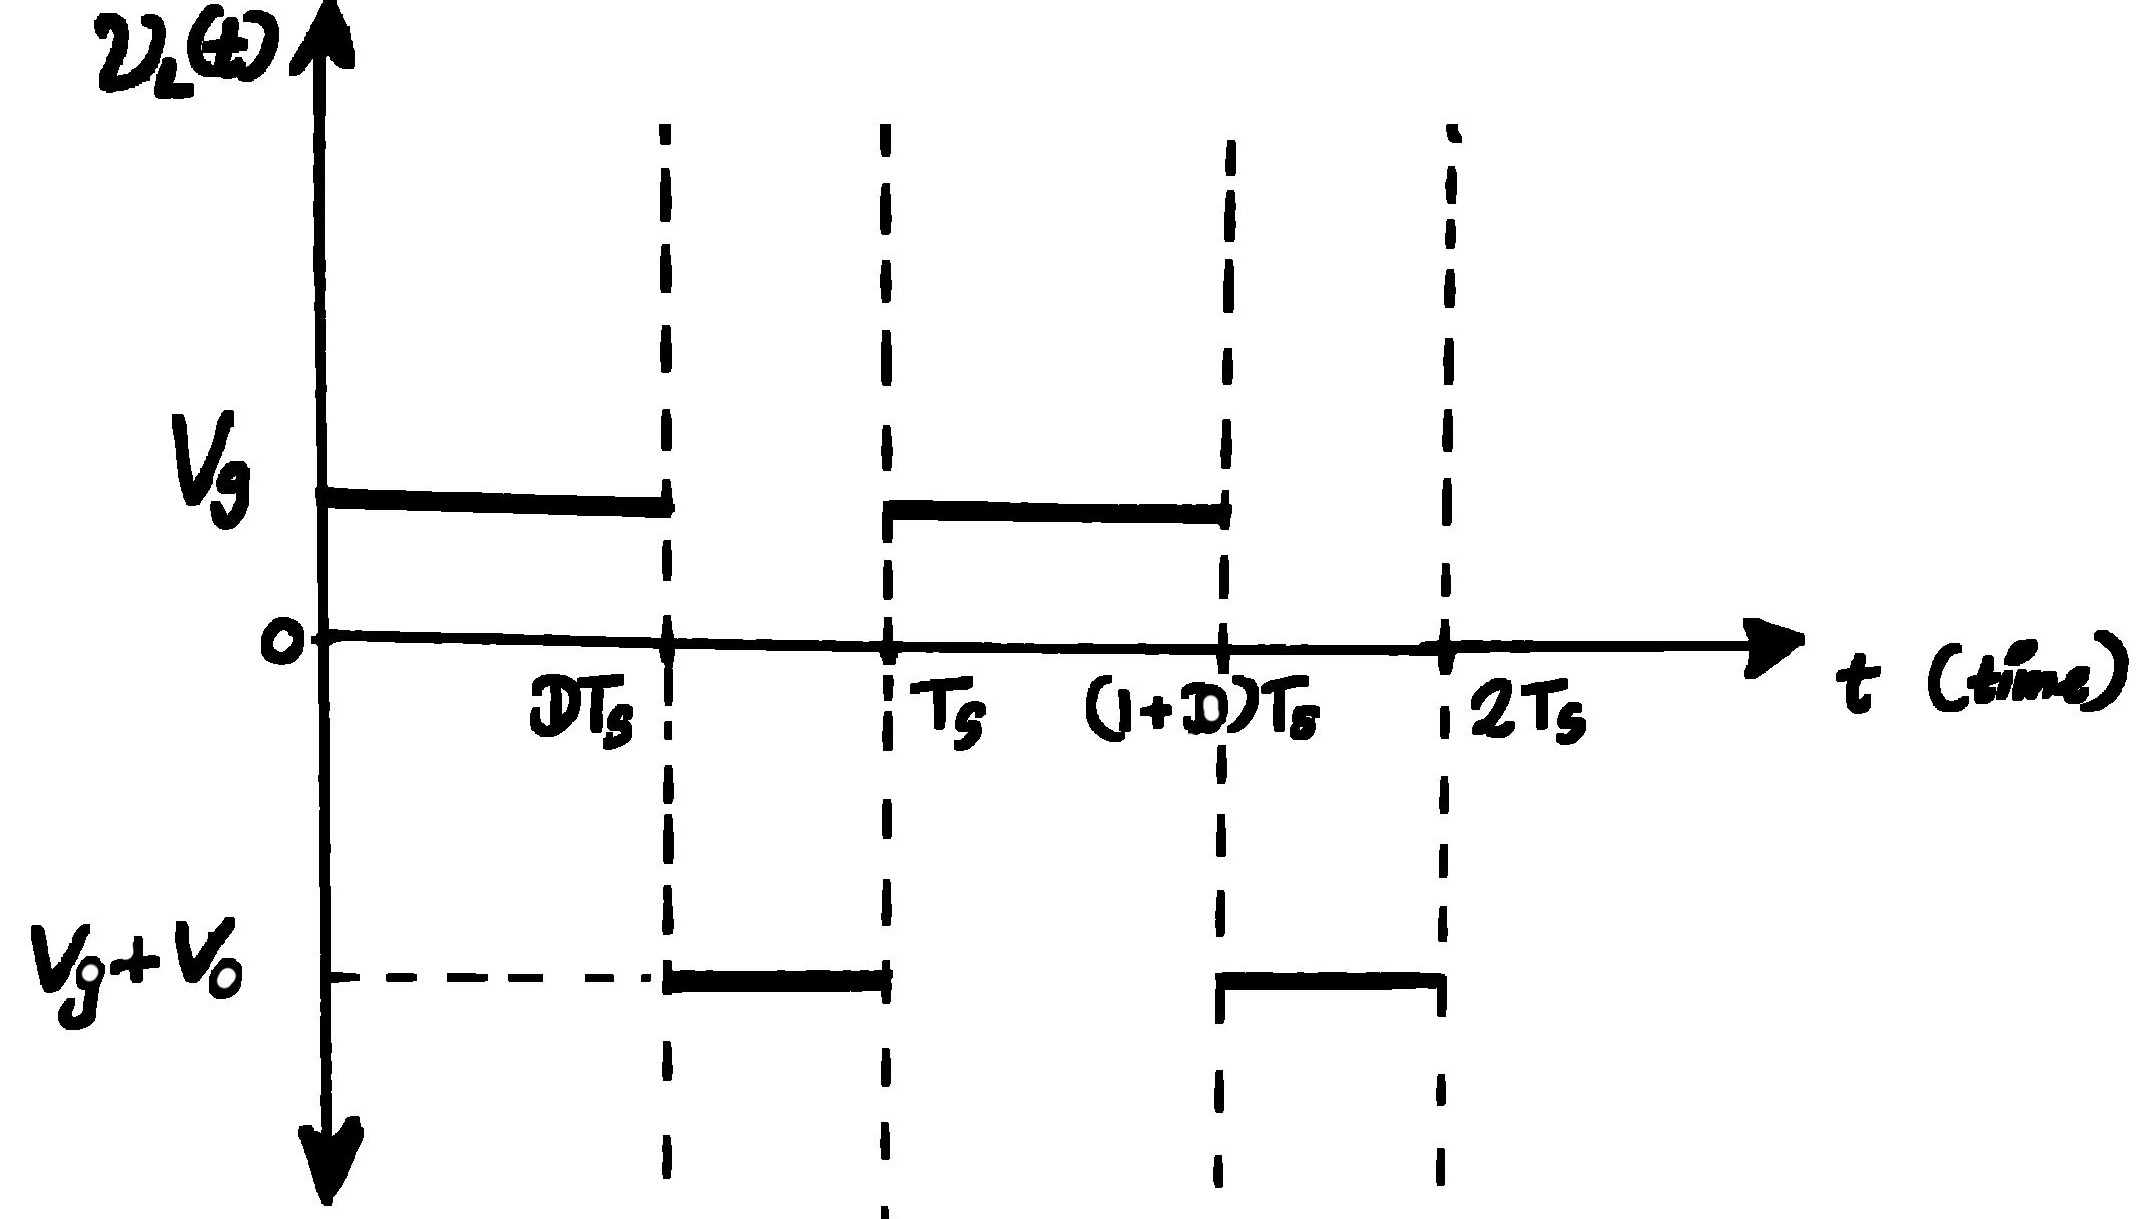
\includegraphics[scale=0.15]{figures/vl}
	\caption{Inductor voltage $v_L(t)$}	
\end{figure}
\pagebreak
Since voltage drop across an inductor is related to the current through it according the following differential equation, graph of the $i_L$ can be directly deduced from the graph of the $v_L$.
\[v_L = L.\frac{d~i_L}{dt}\]

\begin{figure}[!h]
	\centering
	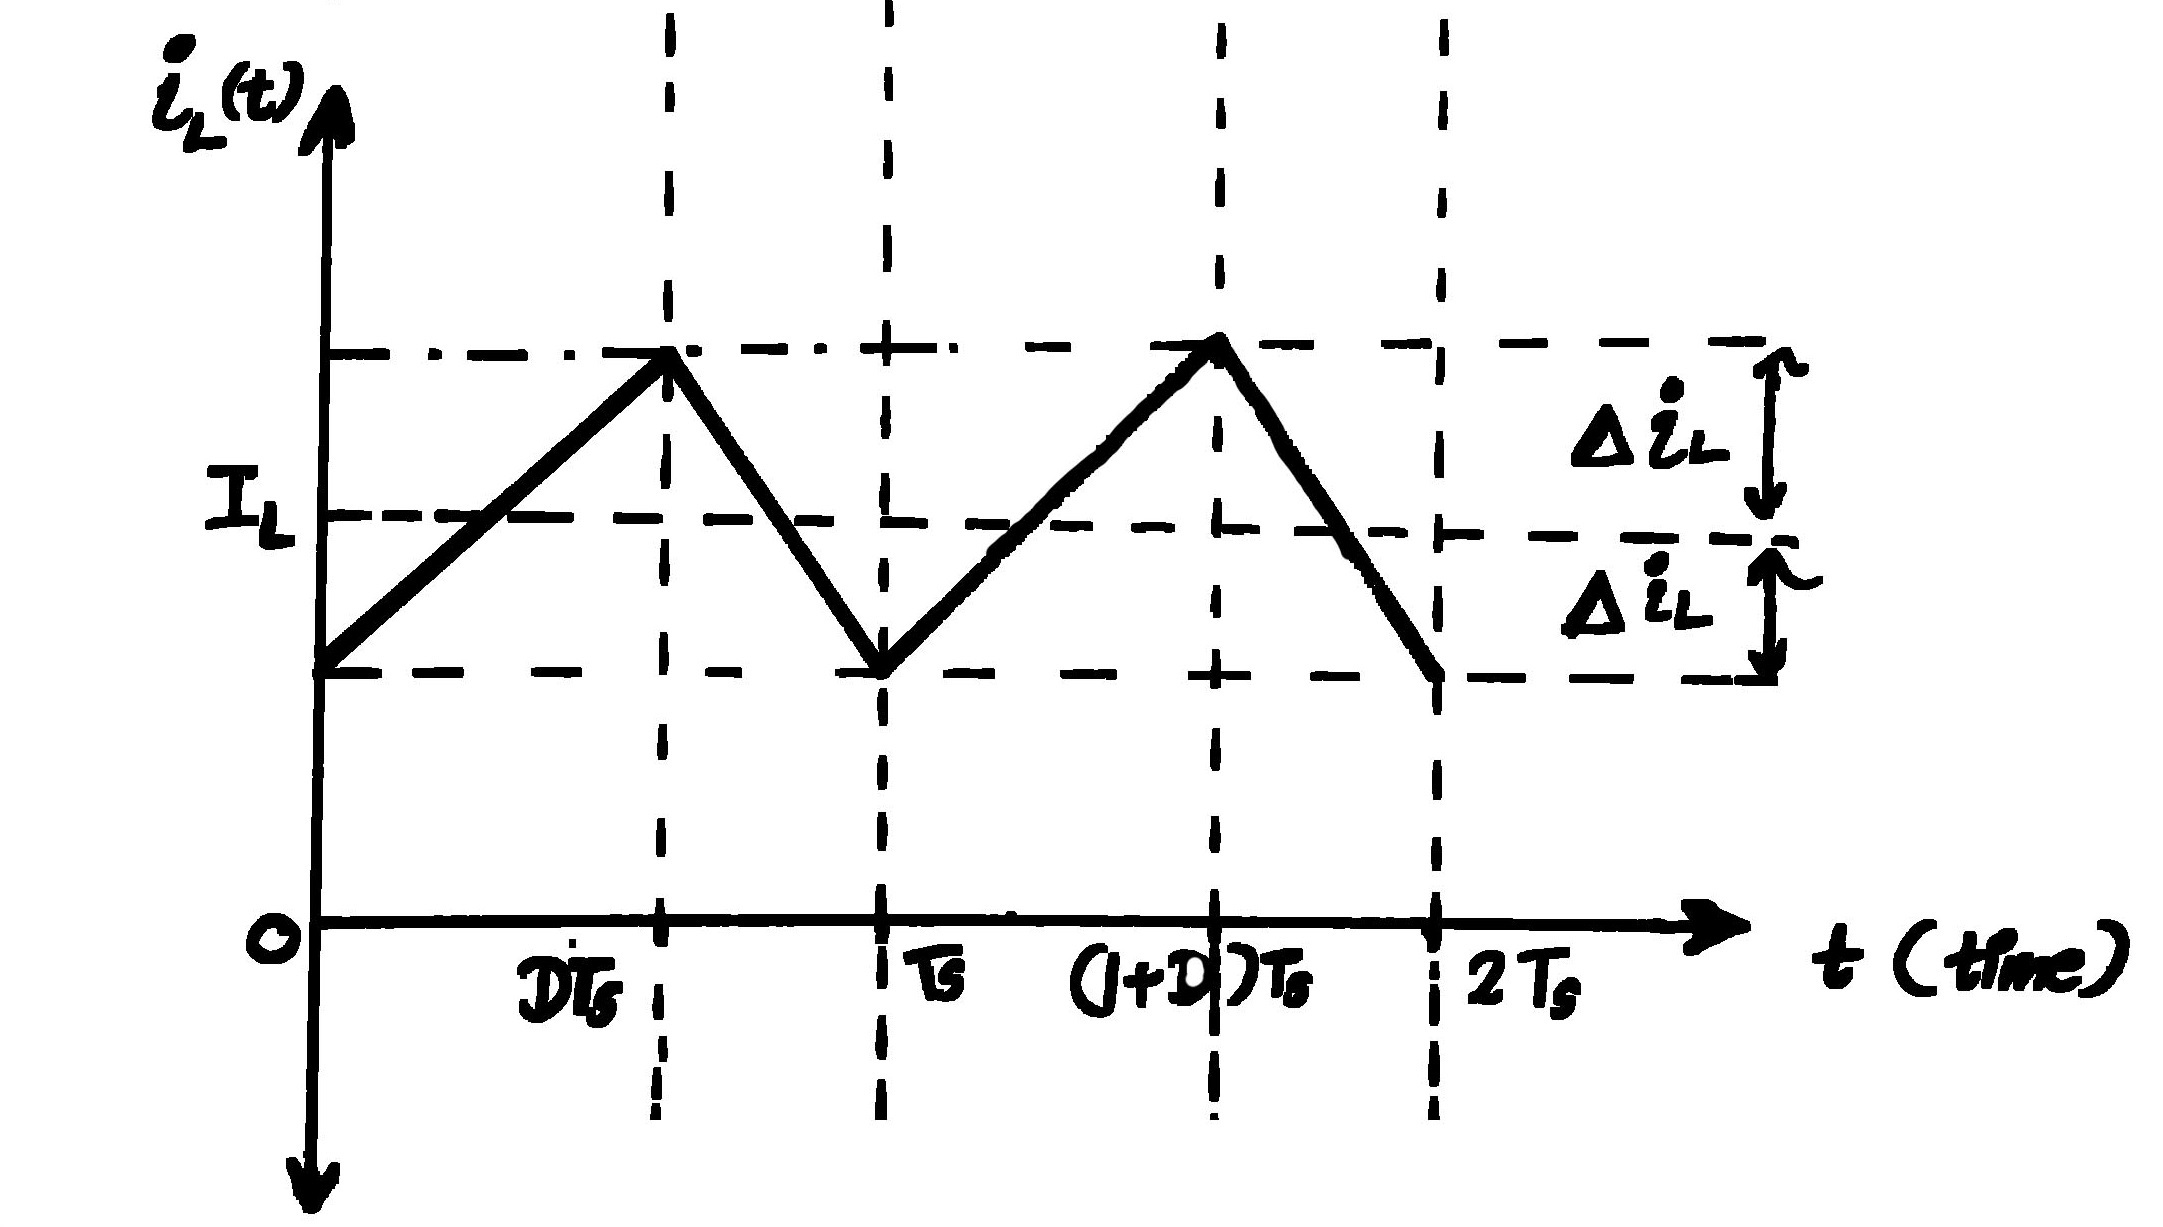
\includegraphics[scale=0.15]{figures/il}	
	\caption{Inductor current $i_L(t)$}
\end{figure}

In the above figure $I_L$ denotes the average inductor current.\\

\hrule
\section*{Q5}
Using inductor volt-second balance,
\[
\begin{split}
	<V_L(t)> = 0 = & \frac{1}{T_s}.\int_{0}^{T_s} V_L(t) ~dt\\
	&=\int_{0}^{DT_s} V_L(t) ~dt + \int_{DT_s}^{T_s}V_L(t) ~dt\\
	&=\int_{0}^{DT_s} V_g  ~dt + \int_{DT_s}^{T_s} V_g + V_o ~dt\\
	&= V_g.DT_s +(V_g + V_o).(T_s - DT_s)\\
	&= V_g.D +(V_g + V_o).(1 - D)\\
	&= V_g + V_o.(1 - D) 
\end{split}
\]

\[\therefore V_o = -\frac{V_g}{1-D}\]

\hrule
\section*{Q6}


\subsection*{S1}
\begin{itemize}
	\item ON Current($i_{S_1}$)	
	
	As described below in the part ``\textbf{S3}'', $i_{S_3}$ is positive in the marked direction. Therefore according to the Kirchhoff Current Low, $i_C + i_{S_3} = 0$ and it implies $i_C$ is negative in the marked direction(actual direction is the opposite of the marked direction). As $v_L$ is positive $i_L$ is positive in the marked direction. Because of these reasons, according to the K.C.L, $i_{S_1} = i_L+(-i_C)$ and it is positive in the marked direction in Fig.\ref{fc}.
%	From Fig.\ref{fc}, using Kirchhoff Current Low, $i_L = i_C + i_{S_1}$. From the calculations of the  Question 04, $v_C = -V_o$. Since $V_o$ is negative, $v_C$ is positive and therefore $i_C$ is positive. While $S_1$ is ON, $v_L = V_g >0$ and therefore $i_L$ is positive. Consider,  $i_L -i_C =  i_{S_1}$
	
	
	\item Blocking Voltage($v_{S_1}$)
	
	From Fig.\ref{sc}, positive and negative terminals of the switch are connected to the positive and negative terminals of the capacitor $C$. Therefore $v_{S_1} = v_C$. 	From the calculations of the  Question 04, $v_C = -V_o$ and $V_o$ is negative. Therefore $v_{S_1}$ is positive.
	
\end{itemize}


\subsection*{S2}
\begin{itemize}
	\item ON Current($i_{S_2}$)	
	
 When considering the loop consist of the Source,inductor, capacitor($C$) and the switch $S_2$ in Fig.\ref{sc}, it is obvious that $i_{S_2}$ is positive in the given direction.
	
%	From the calculations of the  Question 04, $v_C = -V_o$. Since $V_o$ is negative, $v_C$ is positive and therefore $i_C$ is positive. As $i_C = i_{S_2}$ from the Kirchhoff current low(Fig. \ref{sc}),  $i_{S_2}$ is also positive.
	
	
	\item Blocking Voltage($v_{S_2}$)
	
	From Fig.\ref{fc}, $v_{S_2} = v_{C_o} = V_o $. Since $V_o$ is negative, $v_{S_2}$ is also negative.
\end{itemize}


\subsection*{S3}
\begin{itemize}
	\item ON Current($i_{S_3}$)	
	
	Since $V_o~and ~v_{C_o}$ are negative in the marked direction, their currents are also in the direction opposite to the marked direction. Therefore according to the Kirchhoff Current Low, $i_{S_3} = -(i_{C_o} + I_o)$. Which results $i_{S_3}$ to be positive in the marked direction in Fig.\ref{fc}.
%	From Fig.\ref{fc}, using Kirchhoff Current Low, $i_C + i_{S_3} = 0~\therefore i_{S_3} = -i_C$. Since $i_{C}$ is positive in the marked direction, $i_{S_3}$ is positive in the marked direction.
	
	\item Blocking Voltage($v_{S_3}$)
	
	From Fig.\ref{sc}, $v_{S_3} = V_o$ as positive and negative terminals of the switch are connected to the positive and negative terminals of the $R_o$ respectively. Since $V_o$ is negative, $v_{S_3}$ is also negative.
	
\end{itemize}

\begin{table}[!h]
	\centering
	\begin{tabular}{c c c c}
		\textbf{Switch} & \textbf{ON-current} & \textbf{Blocking Voltage} & \textbf{Suitable Semiconductor Device}\\
		S1& $i_{S_1} >0$& $v_{S_1} > 0$& FET\\
		S2& $i_{S_2}>0$ & $v_{S_2} < 0$  & Diode\\
		S3& $i_{S_3}>0$ & $v_{S_3} <0$ & Diode\\
	\end{tabular}
	\caption{Summary of the Proposed Semiconductors according to the catalog developed in the class}
\end{table}

\begin{figure}[!h]
	\centering
	\begin{circuitikz}[american] %, voltage shift=-1
		\ctikzset{inductors/scale=1.5, inductor=cute}
		\draw[thick] (0,0)to[V, l=$V_g$] (0,3) to [L, ,l=$L$, i>=$i_{L}$, 
		v=$v_{L}$](3,3);
		
		\draw[thick]
	 (3,1.5) node[nigfete] (nf) {};
\draw[thick] (nf.D) --(3,3);
\draw[thick] (nf.S) to[short, i>=$i_{S_1}$](3,0);
\draw[thick] (nf.G) node[anchor=east] {$G$};

		%\draw   (3,1.5) node[nigfete] (fet) {}
%		\draw (3,3) to[normal closed switch, l=$S_1$, i>=$i_{S_1}$] 
\draw[thick] (3,0) -- (0,0);
		\draw[thick] (3,3) to[capacitor,l=$C$, i>=$i_{C}$,v=$v_{C}$] (6,3);
		\draw[thick] (6,3) to[D, l=$S_2$,v=$v_{S_2}$, i>=$i_{S_2}$] (6,0) --(3,0);
		\draw[thick] (9,3) to[D, l=$S_3$, i>=$i_{S_3}$,v=$v_{S_3}$](6,3) ;
		\draw[thick] (9,3) to[capacitor,l=$C_o$, i>=$i_{C_o}$,v=$v_{C_o}$] (9,0)--(6,0);
		\draw[thick](9,3) --(12,3) to[R=$R_o$, v=$V_o$, i>=$I_{o}$](12,0) -- (9,0);
	\end{circuitikz}
	\caption{Final Switching Circuit with the Proposed Semiconductors: The control signal is supplied to the Gate terminal($G$) of the FET.}

\end{figure}

\end{document}
